% ===== Indirect-feedback RAG =====
\section{Indirect Feedback for Retrieval-Augmented Generation}
\label{sec:mm_rag}

Dense retrievers are usually trained from passage-level relevance labels. We instead optimize a
retriever by the success of the reader that consumes its output: a passage is useful when a frozen
reader can answer the question from it. This replaces direct relevance supervision with the
downstream signal of interest and requires only question--answer pairs. We evaluate the same
principle in text-only retrieval and in multimodal retrieval, where the query contains an image and
a question.

\subsection{Method}
\label{sec:rag_method}

For a query $q$ and passage $d$, the retriever assigns
$s_\theta(q,d)=\langle e_\theta(q),e_\theta(d)\rangle/\tau$. We form a support
$\mathcal{M}_q$ from the policy's top-$M$ passages and sample an ordered list
$D=(d_1,\ldots,d_k)$ without replacement. Its exact Plackett--Luce log-probability is
\begin{equation}
\log \pi_\theta(D\mid q)
=\sum_{i=1}^{k}\left[s_\theta(q,d_i)
-\log\!\sum_{d\in\mathcal{M}_q\setminus\{d_1,\ldots,d_{i-1}\}}
\exp s_\theta(q,d)\right].
\label{eq:pl}
\end{equation}
This factorization matches Gumbel-top-$k$ sampling and accounts for the shrinking support after each
selection.

A frozen reader answers the question from each sampled passage. If
$y_n\sim\operatorname{Reader}(\cdot\mid q,d)$ is one of $N$ sampled answers and
$\mathcal{A}^{\star}$ is the answer-alias set, the passage and list rewards are
\begin{equation}
r(q,d)=\frac{1}{N}\sum_{n=1}^{N}
\mathbf{1}\!\left[y_n\text{ matches an }a\in\mathcal{A}^{\star}\right],
\qquad
R(D)=\frac{1}{k}\sum_{i=1}^{k}r(q,d_i).
\label{eq:reward}
\end{equation}
For each query we draw $G$ lists and standardize their rewards within the group,
$\hat A_g=(R(D_g)-\mu_R)/(\sigma_R+\epsilon)$. The retriever is updated with
\begin{equation}
\mathcal{J}(\theta)=
\mathbb{E}\!\left[\frac{1}{G}\sum_{g=1}^{G}
\hat A_g\log\pi_\theta(D_g\mid q)\right],
\label{eq:rag_objective}
\end{equation}
which is REINFORCE with a within-query group baseline, following the group-relative principle of
GRPO~\citep{shao2024deepseekmath}. No critic, relevance label, annotated positive passage,
contrastive loss, or reference-policy penalty enters the finalized objective. The multimodal
configuration uses $M{=}24$, $k{=}4$, and $G{=}4$; the text configuration uses the same listwise
objective with setting-specific list and support sizes.

% Method figure for v3-pure (fig_mm_v3_arch.pdf) — the working annotation-free loop.
% Companion to fig_af_rl_arch (the v1 recipe); same blue/orange convention:
%   BLUE = trainable retrieval path, ORANGE = frozen reward path.
%
% REPRO(fig:mm-v3-arch): both artifacts come from ONE layout spec so they cannot drift:
%   MMRAG_DATA=<data> python3 mmrag/plot_v3_arch.py --out mmrag/fig_mm_v3_arch
% It emits the edge-trimmed PDF (bbox_inches=tight) AND the editable fig_mm_v3_arch.pptx.
% Every hyperparameter on the figure is read from $MMRAG_DATA/runs/v3-pure/args.json at draw
% time — a missing key is a hard error, and the script refuses to draw a run that is not
% v3-pure (asserts algo=plgrpo, contrastive_coef=0, no_force_gold). The backbone name is parsed
% out of encoder.py:ENCODER_PROFILES, NOT derived from the reader (an earlier draft printed
% "Qwen2.5-VL-2B" for what is a Qwen2-VL encoder). A renderer bbox check measures every text
% extent against its owning box and reports violations; current status 0.
%
% NOTE the PDF is drawn by matplotlib from the shared spec rather than converted from the PPTX:
% this machine has no LibreOffice/soffice/unoconv. Re-export the PPTX through PowerPoint if a
% literally-converted PDF is wanted; the geometry is identical because both come from build_spec().
%
% Box -> code (VLM2Vec-rl @ v23-base): query/index train_rl.build_rl_corpus + refresh_corpus();
% policy encoder.load_encoder + rl_core.pool_logps; sampling rl_core.pl_sample_lists /
% pl_list_logps; reward reader_vlm.score_judge -> answer_correct; credit train_rl.main
% (R.mean over the list, z-score over G) + rl_core.embedding_ppo_loss.
\begin{figure}[t]
\centering
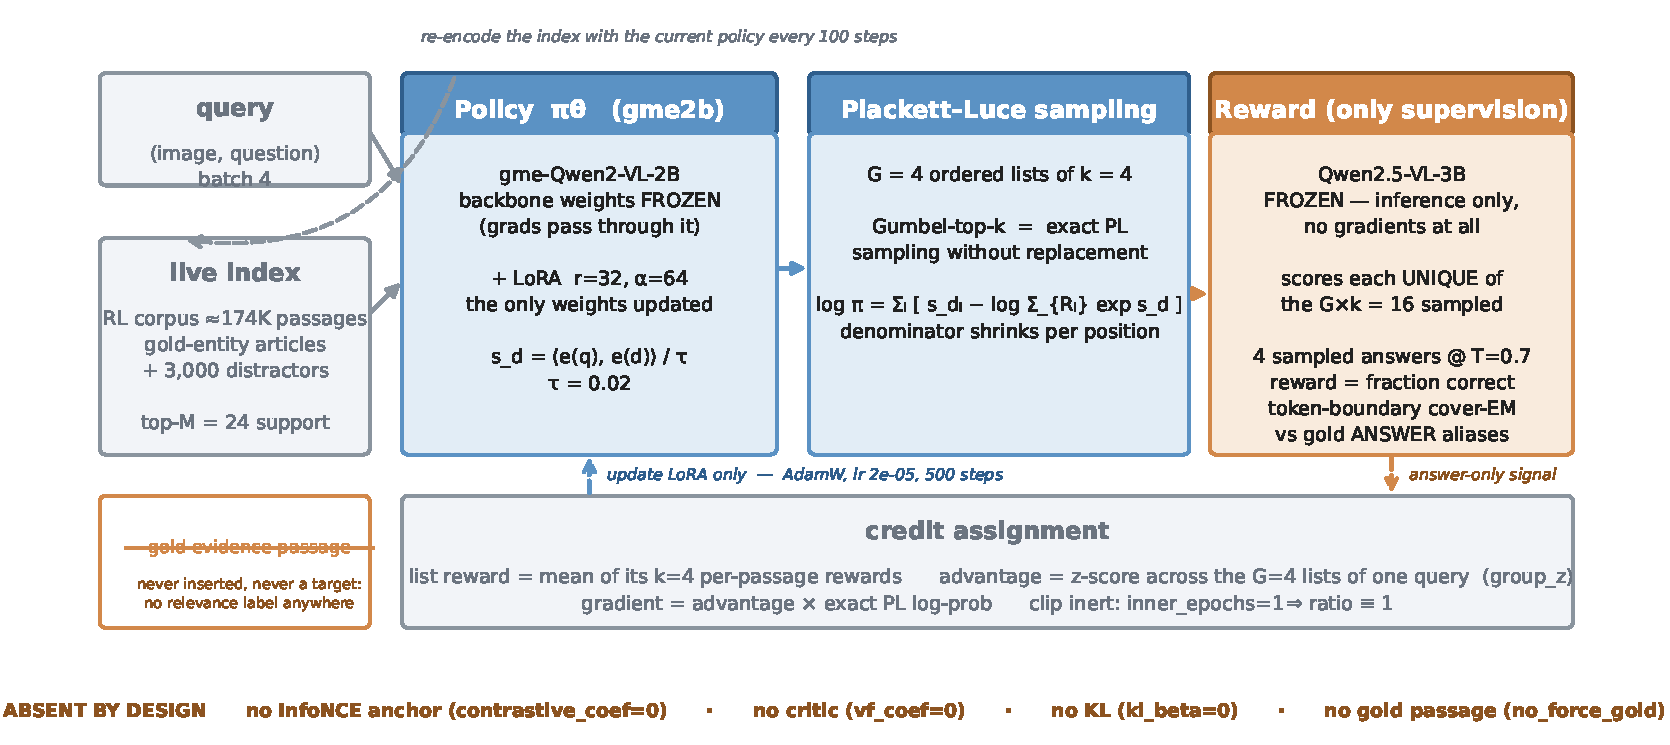
\includegraphics[width=\linewidth]{fig_mm_v3_arch.pdf}
\caption{\textbf{Training architecture of \textsc{v3-pure}, the working annotation-free loop.}
The retriever policy $\pi_\theta$ (\textsc{GME-Qwen2-VL-2B}; LoRA $r{=}32$, $\alpha{=}64$ are the
only trainable parameters) scores an image--question query against a \emph{live} index that is
re-encoded with the current policy every $100$ steps. An action is an ordered list of $k{=}4$
passages; $G{=}4$ such lists are drawn per query by Gumbel-top-$k$ over the policy's own top-$24$
support, which is exact Plackett--Luce sampling without replacement, and scored by the exact
conditional factorisation whose denominator shrinks at each position. A \emph{frozen}
\textsc{Qwen2.5-VL-3B} reader scores each unique sampled passage once, sampling $4$ answers at
$T{=}0.7$; the reward is the fraction that match a gold answer alias under token-boundary
cover-EM. List rewards are $z$-scored across the $G$ lists of a query, and the update is the
advantage-weighted exact log-probability --- with one inner epoch the PPO ratio is identically
one, so the clip never engages. Blue marks the trainable retrieval path, orange the frozen reward
path. What is \emph{absent} is the method's point: no InfoNCE anchor, no critic, no KL penalty,
and no gold passage --- the annotated evidence passage is never inserted into a pool and is never
a target, so the only supervision anywhere in the loop is the gold \emph{answer} string inside
the reward. Every hyperparameter shown is read from the shipped run's \texttt{args.json}; an
editable copy ships as \texttt{fig\_mm\_v3\_arch.pptx}.}
\label{fig:mm-v3-arch}
\end{figure}


\subsection{Experimental Setup}
\label{sec:rag_setup}

\paragraph{Text retrieval.}
We train a \textsc{Qwen3-Embedding-0.6B} retriever on an eleven-source QA mixture. The reader's
answer correctness is the only reward. We report in-domain $R@5$ and zero-shot transfer on five
BEIR domains (SciFact, NFCorpus, ArguAna, FiQA, and SciDocs), summarized by mean nDCG@$10$.

\paragraph{Multimodal retrieval.}
We train \textsc{GME-Qwen2-VL} retrievers at 2B and 7B scale on InfoSeek image--question--answer
triples. All trained arms use the same LoRA adapter budget ($r{=}32$, $\alpha{=}64$). Retrieval is
evaluated over a $422{,}378$-passage Wikipedia corpus on $3{,}000$ queries. Downstream VQA accuracy
uses a frozen \textsc{Qwen2.5-VL-7B} reader over the top five passages on $1{,}500$ queries. For
out-of-domain evaluation, InfoSeek-trained retrievers are transferred to Encyclopedic-VQA without
additional training.
We also test robustness to index composition by scoring the frozen base encoder and both trained
arms against the homogeneous evaluation pool and against a $2$M-passage mixed-domain index.

\paragraph{Baselines and metrics.}
In both modalities we compare against the untrained base retriever and a data-matched relevance-SFT
baseline that directly observes positive passages. We report entity recall, which credits passages
from the gold entity, answer recall, which requires an answer-bearing passage, and downstream answer
accuracy. InfoSeek numeric-range answers are graded by whether a predicted number lies inside the
provided tolerance; all other answers use token-boundary cover exact match. This corrects a benchmark
implementation that otherwise assigns all numeric-range items a zero.

\subsection{Main Results}
\label{sec:rag_results}


Table~\ref{tab:mm_main} compares the finalized retriever with the base and relevance-SFT controls;
development variants appear only in the ablations.

\begin{table}[H]
\centering\small
\caption{In-domain text retrieval and multimodal VQA (\%). The text row is the finalized full-data
run. Multimodal $\pm$ is sample SD over three seeds at 2B and two seeds for our 7B model; 7B SFT
has one seed. Results from different datasets are not directly comparable.}
\label{tab:mm_main}
\begin{tabular}{llccc}
\toprule
setting & metric & base & relevance-SFT & ours \\
\midrule
text, 0.6B & $R@5$ & 66.9 & \textbf{83.8} & 78.7 \\
\midrule
multimodal, 2B & VQA accuracy & 38.40 & $41.22 \pm 1.47$ & $\mathbf{43.44 \pm 0.34}$ \\
               & entity $R@5$ & 68.53 & $75.16 \pm 0.58$ & $\mathbf{76.09 \pm 1.02}$ \\
               & answer $R@5$ & 54.94 & $61.96 \pm 1.35$ & $\mathbf{63.46 \pm 0.95}$ \\
\midrule
multimodal, 7B & VQA accuracy & 39.67 & 41.60 & $\mathbf{45.23 \pm 0.33}$ \\
               & entity $R@5$ & 69.37 & 77.67 & $\mathbf{80.63 \pm 0.47}$ \\
               & answer $R@5$ & 53.59 & 63.02 & $\mathbf{68.71 \pm 0.43}$ \\
\bottomrule
\end{tabular}
\end{table}

\clearpage
\input{fig_rag_budget}

\paragraph{Text retrieval improves substantially without relevance labels.}
Indirect feedback raises in-domain $R@5$ from $66.9$ to $78.7$ without relevance labels, while
relevance-SFT reaches $83.8$ (Table~\ref{tab:mm_main}). In the separate frozen-index budget study,
SFT reaches $64.5$ with $1.3$K labeled rows; indirect feedback reaches $64.3$ after $25$K
question--answer examples (Fig.~\ref{fig:rag_budget}). Thus the label-free gain does not imply
greater sample efficiency. Exact checkpoints and SFT tuning are in App.~\ref{app:rl_budget}.

\paragraph{Multimodal retrieval matches or beats relevance-SFT.}
At 2B, indirect feedback improves downstream accuracy by $2.22$ points over SFT, with every
indirect-feedback seed above every SFT seed; a paired per-query test gives
$p=2.8\times10^{-5}$. Entity and answer $R@5$ improve by $0.93$ and $1.50$ points, respectively,
but their seed intervals overlap, so we treat retrieval as a tie at this scale. At 7B, the indirect
retriever leads SFT on all three metrics: $+3.63$ accuracy, $+2.96$ entity $R@5$, and $+5.69$
answer $R@5$. The central comparison is therefore consistent across scale: optimizing reader
success is at least as effective as direct relevance supervision, and its advantage is clearest on
the downstream objective.

\paragraph{A larger, mixed-domain index.}
Adding cross-domain distractors enlarges the index $4.7\times$ and lowers the frozen encoder's
entity $R@5$ from $68.53$ to $14.27$. Both trained retrievers retain about $69$\% recall
(Table~\ref{tab:rag_mixed_domain}); their $0.76$-point gap is smaller than the $2.03$-point pooled
between-seed variation measured on these queries. Indirect feedback nevertheless retains a
downstream lead on the larger index:
answer $R@5$ is $57.88$ versus $54.49$, and accuracy is $41.93$ versus $36.47$
(Table~\ref{tab:mm_ood_summary}). The large gain over the frozen encoder reflects training under
either objective, not a unique effect of indirect feedback. A relaxed check that credits any passage
about the correct entity still leaves the frozen encoder far behind
(App.~\ref{app:mm_credit}).

\begin{table}[H]
\centering\small
\caption{Entity $R@5$ (\%) on the same InfoSeek queries as the index grows from $422$K to $2$M
passages. Each row uses the same single-seed models.}
\label{tab:rag_mixed_domain}
\begin{tabular}{lccc}
\toprule
evaluation index & base & relevance-SFT & ours \\
\midrule
InfoSeek, $422$K passages      & $68.53$ & $73.17$ & $\mathbf{75.83}$ \\
InfoSeek, mixed $2$M passages  & $14.27$ & $69.07$ & $\mathbf{69.83}$ \\
\bottomrule
\end{tabular}
\end{table}

\paragraph{Out-of-domain evaluation.}
The text models transfer without training on any BEIR evaluation set; the evaluated retriever
re-encodes each corpus. Multimodal models train only on InfoSeek. Encyclopedic-VQA changes the
queries, images, and corpus; the mixed-index test changes only InfoSeek's passage pool. We show both
the in-domain-selected SFT checkpoint and its endpoint, and indirect retrievers trained on the
$422$K and $2$M indexes.

\begin{table}[H]
\centering\small
\caption{Zero-shot text retrieval on BEIR datasets unseen in training (nDCG@$10$). The mean
covers the five primary domains; three further domains provide an additional transfer check.}
\label{tab:rag_ood_text_beir}
\begin{tabular}{lccc}
\toprule
dataset & base & relevance-SFT & ours \\
\midrule
SciFact & $0.694$ & $0.527$ & $0.702$ \\
NFCorpus & $0.358$ & $0.220$ & $0.358$ \\
ArguAna & $0.484$ & $0.323$ & $0.472$ \\
FiQA & $0.429$ & $0.198$ & $0.437$ \\
SciDocs & $0.228$ & $0.123$ & $0.225$ \\
\midrule
mean (five domains) & $0.439$ & $0.278$ & $0.439$ \\
\midrule
TREC-COVID & $0.800$ & $0.486$ & $0.856$ \\
Touch\'e-2020 & $0.227$ & $0.191$ & $0.253$ \\
Quora & $0.856$ & $0.020$ & $0.869$ \\
\bottomrule
\end{tabular}
\end{table}


\begin{table}[H]
\centering\small
\caption{Out-of-domain multimodal results (\%). Accuracy uses a frozen reader on $1{,}500$
queries; recalls use $2{,}701$ Encyclopedic-VQA or $3{,}000$ InfoSeek queries. Domain-shift
results show sample SD for our three seeds; mixed-index rows use one seed.}
\label{tab:mm_ood_summary}
\begin{tabular}{lccc}
\toprule
model & VQA accuracy & entity $R@5$ & answer $R@5$ \\
\midrule
\multicolumn{4}{l}{\emph{InfoSeek $\rightarrow$ Encyclopedic-VQA}} \\
base (frozen) & $42.07$ & $76.31$ & $64.84$ \\
relevance-SFT (selected) & $43.47$ & $78.38$ & $66.73$ \\
relevance-SFT (endpoint) & $39.33$ & $71.05$ & $55.71$ \\
ours & $44.67\pm1.27$ & $80.23\pm1.21$ & $68.48\pm3.55$ \\
\midrule
\multicolumn{4}{l}{\emph{InfoSeek, $422$K $\rightarrow$ mixed-domain $2$M index}} \\
base (frozen) & $25.13$ & $14.27$ & $9.96$ \\
relevance-SFT & $36.47$ & $69.07$ & $54.49$ \\
ours (trained on $422$K) & $41.93$ & $69.83$ & $57.88$ \\
ours (trained on $2$M) & $41.93$ & $69.67$ & $56.82$ \\
\bottomrule
\end{tabular}
\end{table}

\paragraph{Out-of-domain transfer retains a downstream lead.}
Across five BEIR domains, indirect feedback retains the base model's mean nDCG@$10$ of $0.439$,
whereas relevance-SFT falls to $0.278$. Indirect feedback stays within $0.012$ of the base on each
domain, while SFT declines on all five (Table~\ref{tab:rag_ood_text_beir}). The three additional
BEIR sets show the same ordering.


On Encyclopedic-VQA, indirect feedback reaches $44.67\pm1.27$ accuracy and $80.23\pm1.21$ entity
$R@5$, above the base by $2.60$ and $3.92$ points and above the in-domain-selected SFT checkpoint
by $1.20$ and $1.85$ points. The SFT endpoint is weaker still. On the $2$M index, the
$422$K-trained indirect model matches the one trained on that index ($41.93$ accuracy for both;
$69.83$ versus $69.67$ entity $R@5$), so the downstream gain does not require training against the
added distractors (Table~\ref{tab:mm_ood_summary}).

\subsection{Ablation and Analysis}
\label{sec:rag_ablation}

\paragraph{Objective components.} We first test whether standard policy-optimization additions account for the gain. Entropy
regularization, an RLOO baseline, a KL penalty, and their combination all fail to improve the
finalized objective (Table~\ref{tab:mm_v3add}); the simplest group-baseline update is therefore our
default.

\begin{table}[H]
\centering\small
\caption{Objective ablations on InfoSeek VQA accuracy. Each variant adds the indicated component to
our finalized objective; single seed unless noted.}
\label{tab:mm_v3add}
\begin{tabular}{lcc}
\toprule
variant & VQA accuracy (\%) & $\Delta$ \\
\midrule
\textbf{ours} & $\mathbf{43.44 \pm 0.34}$ (3 seeds) & --- \\
$+$ entropy & $43.17$ (2 seeds) & $-0.27$ \\
$+$ RLOO & $42.67$ & $-0.77$ \\
$+$ KL & $41.60$ & $-1.84$ \\
$+$ all & $39.40$ & $-4.04$ \\
\bottomrule
\end{tabular}
\end{table}

\paragraph{Live-index refresh.} Refreshing passage embeddings helps early multimodal training, but
the gap largely closes by $6$K queries (Table~\ref{tab:ab_refresh}). Text retrieval shows no uniform
winner across corpus sizes.

\begin{table}[H]
\centering\scriptsize
\setlength{\tabcolsep}{4.2pt}
\caption{Compact live-index ablation. Differences are frozen minus refreshed; negative values favor
refreshing. Text rows report query-tower $R@5$.}
\label{tab:ab_refresh}
\begin{tabular}{llccc}
\toprule
setting & metric & refreshed & frozen & difference \\
\midrule
multimodal, $3$K & answer $R@5$ & $65.65 \pm 0.55$ & $61.43$ & $-4.22$ \\
multimodal, $3$K & accuracy & $43.03 \pm 0.71$ & $39.40$ & $-3.63$ \\
multimodal, $6$K & answer $R@5$ & $65.37 \pm 1.76$ & $65.51$ & $+0.14$ \\
multimodal, $6$K & accuracy & $44.50 \pm 1.27$ & $43.47$ & $-1.03$ \\
text, $50$K corpus & $R@5$ & $77.4 \pm 1.7$ & $76.0 \pm 1.3$ & $-1.4$ \\
text, $200$K corpus & $R@5$ & $65.3 \pm 0.7$ & $66.9 \pm 3.3$ & $+1.6$ \\
text, $1$M corpus & $R@5$ & $60.8$ & $57.8$ & $-3.0$ \\
\bottomrule
\end{tabular}
\end{table}

\paragraph{Retriever initialization and optimization.} Indirect feedback learns reliably from the
strong GME starts, while weaker starts can regress; even the same BGE backbone changes sharply with
learning rate (Table~\ref{tab:ab_init}). This is a scope condition rather than a headline comparison.
The broader backbone and learning-rate checks are in
App.~Tables~\ref{tab:mm_backbone} and~\ref{tab:mm_lr}.

\begin{table}[H]
\centering\scriptsize
\setlength{\tabcolsep}{3.6pt}
\caption{Representative initialization and optimization results. Multimodal rows report entity
$R@5$; text rows report reader accuracy. Results are percentages and use one seed unless noted.}
\label{tab:ab_init}
\begin{tabular}{llllrrr}
\toprule
modality & backbone & lr & metric & base & indirect & $\Delta$ \\
\midrule
multimodal & GME-Qwen2-VL-7B & $1\!\times\!10^{-5}$ & entity $R@5$ & $69.37$ & $80.97$ & $+11.60$ \\
multimodal & GME-Qwen2-VL-2B & $2\!\times\!10^{-5}$ & entity $R@5$ & $68.53$ & $75.27$ & $+6.73$ \\
multimodal & BGE-VL-large & $1\!\times\!10^{-5}$ & entity $R@5$ & $15.73$ & $21.23$ & $+5.50$ \\
multimodal & BGE-VL-large & $1\!\times\!10^{-4}$ & entity $R@5$ & $15.73$ & $0.70$ & $-15.03$ \\
multimodal & VLM2Vec-7B & $2\!\times\!10^{-5}$ & entity $R@5$ & $14.37$ & $2.90$ & $-11.47$ \\
text & MiniLM-L6 & fixed & reader acc. & $67.6$ & $63.8$ & $-3.8$ \\
text & Harrier-27B & fixed & reader acc. & $76.0$ & $77.6$ & $+1.6$ \\
\bottomrule
\end{tabular}
\end{table}

\paragraph{Text training mixture.} The in-domain gain persists across source compositions, while
BEIR remains near the $0.439$ base (Table~\ref{tab:ab_datamix}). We use the natural eleven-source
mix for coverage rather than selecting the best mixture post hoc.

\begin{table}[H]
\centering\scriptsize
\setlength{\tabcolsep}{8pt}
\caption{Representative text-mixture results under the same $50$K index and $6$K-query recipe.}
\label{tab:ab_datamix}
\begin{tabular}{lcc}
\toprule
training mix & in-domain $R@5$ & BEIR nDCG@$10$ \\
\midrule
base encoder & $66.9$ & $0.439$ \\
natural eleven-source mix & $77.4$ & $0.439$ \\
web QA & $78.0$ & $0.440$ \\
reading/science & $77.3$ & $0.438$ \\
MS MARCO only & $72.7$ & $0.437$ \\
NQ only & $72.5$ & $0.436$ \\
\bottomrule
\end{tabular}
\end{table}

\paragraph{Reward informativeness.} A gold/no-gold reader check finds usable reward on roughly one
third of training queries in both modalities (Table~\ref{tab:ab_reward}). Offline filtering improves
text $R@5$ against a size-matched control. Online masking instead raises multimodal entity $R@5$
while reducing answer $R@5$ and accuracy, reinforcing the distinction between entity overlap and
reader utility. The reader-outcome breakdown and matched mask results are in
App.~Tables~\ref{tab:rag_mech} and~\ref{tab:rag_mask}.

\begin{table}[H]
\centering\small
\caption{Reward availability and filtering controls. Usable share is measured on training queries;
filter and mask effects are percentage-point changes from matched controls.}
\label{tab:ab_reward}
\begin{tabular}{llr}
\toprule
setting & measure & result \\
\midrule
text & usable queries & $36.9\%$ \\
image + text & usable queries & $33.9\%$ \\
text offline filter & $\Delta R@5$ & $+2.75$ \\
multimodal online mask & $\Delta$ entity $R@5$ & $+1.07$ \\
 & $\Delta$ answer $R@5$ & $-3.49$ \\
 & $\Delta$ VQA accuracy & $-2.00$ \\
\bottomrule
\end{tabular}
\end{table}
